\documentclass[12pt, a4paper]{article}
\usepackage{../../../../../style}
\begin{document}
	
\lhead{Группа 102} \chead{Модуль 6 Занятие №3} \rhead{Школа <<Симметрия>>}
\section{Построение сечений}
\begin{enumerate}
	\item Постройте сечение треугольной призмы $ABCA_1B_1C_1$ плоскостью, проходящей через центр грани $AA_1B_1B$, середину ребра $B_1C_1$ и точку $M$ ребра $A_1C_1$,
	если $A_1M:MC_1=1 : 2$.
	\item Основание пирамиды $SABCD$ --- параллелограмм $ABCD$. Постройте сечение пирамиды плоскостью, проходящей через следующие точки:
	\begin{enumerate}[label=\asbuk*)]
		\item середины рёбер $AD$, $SC$ и точку $B$;
		\item центр основания, середину ребра $SD$ и точку $M$ ребра $SA$, если $AM :MS = 1 : 3$.
	\end{enumerate}
\end{enumerate}
\section{Угол между прямой и плоскостью}
	Углом между прямой и плоскостью называется угол между прямой
	и её ортогональной проекцией на плоскость.
	\begin{center}
		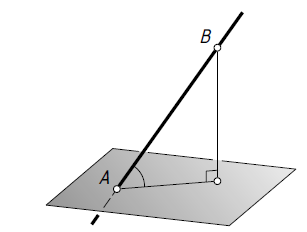
\includegraphics[width=0.3\textwidth]{pic_1}
	\end{center}
	\begin{enumerate}
		\item Дан куб $ABCDA_1B_1C_1D_1$. Найдите углы:
		\begin{enumerate}[label=\asbuk*)]
			\item между прямой $AC_1$ и плоскостью $BDD_1$;
			\item между прямой $AC$ и плоскостью $BCD_1$.
		\end{enumerate}
		\item В правильной четырёхугольной пирамиде $SABCD$ апофема равна стороне основания. Найдите угол между плоскостью $CSD$ и апофемой пирамиды, содержащейся в плоскости $ASB$.
		\item Дана правильная четырёхугольная пирамида $SABCD$ с вершиной $S$. Все рёбра пирамиды равны, $M$ --- середина бокового ребра $SD$. Найдите угол между прямой $AM$ и плоскостью $ABC$.
		\item Дана правильная треугольная призма $ABCA_1B_1C_1$, все рёбра которой равны $1$. Точка $M$ --- середина ребра $BC$. Найдите угол между прямой $C_1M$ и плоскостью $ABB_1$.
	\end{enumerate}
\end{document}